\section{Experiments}
\label{sec:exp}

In this section, we conduct experiments to
(1) examine the performance of our two-stream PsyEx model compared with strong baselines; (2) validate the effectiveness of various design choices with ablation tests; (3) evaluate the model's generalizability on different datasets; 
(4) analyze the interpretability enabled by symptoms and disease-specific 
``experts''. 
% \MY{Why are you ordering the diseases in Table 1,2 in this way? Consider a logical order i.e. from diseases with most users to least}

\begin{table*}[th]
    \small
    \centering
    \begin{tabular}{l|ccccccc|c}
    \hline
    Method & Depression & Anxiety & ADHD & Bipolar & OCD & PTSD & Eating & Avg. F1 \\ 
    \hline
    TF-IDF+LR \cite{cohan2018smhd} & 76.75	&75.45	&68.97	&76.56	&40.0	&44.02	&30.0 &	58.82 \\
    BERT \citep{nguyen2022improving} & 73.28&	70.59&	56.72&	61.21&	41.82&	50.0&	32.67 &	55.18 \\
    Symp \citep{Zhang2022SymptomIF} & 81.06 &	81.99&	70.3&	81.75&	65.12&	64.41&	61.54 &	72.31  \\
    HAN-GRU \citep{sekulic2019adapting}& 74.99&	82.16&	81.72&	80.28&	70.59&	67.67&	68.57&	75.14   \\
    ChatGPT & 70.12	&73.09	&64.08	&67.12	&52.98	&67.61	&29.73	&60.68  \\ 
    \hline
    PsyEx & \textbf{87.89}&    \textbf{89.84}&	\textbf{84.40}&	\textbf{91.58}&	\textbf{81.69} &	\textbf{81.69}&	\textbf{85.71}&	\textbf{86.12} \\ 
    \hline
    \end{tabular}
    \caption{Mental Disease Detection Results across 7 diseases on Reddit dataset, reporting F1 scores in binary setting. We order these diseases in descending order according to their number of patients in the dataset, making it easier to identify rarer classes.}
    \label{tab:disease}
\end{table*}

\begin{table*}[th]
    \small
    \centering
    \begin{tabular}{l|ccccccc|cc|c}
    \hline
    Method & Depression & Anxiety & ADHD & Bipolar & OCD & PTSD & Eating &  macro-F1 & micro-F1 & EM \\ 
    \hline
    TF-IDF+LR & 52.16& 32.52& 29.9&	43.14&	13.79&	9.76 & 	0& 25.9&38.09&	77.37  \\
    BERT & 56.99&	47.03&	31.86&	16.59&	0&	0&	0 & 21.78& 39.38&	75.32  \\
    Symp & 62.99&	\textbf{57.93}&	49.57&	51.85&	18.18&	0&	0& 34.36& 53.05&	76.65   \\
    HAN-GRU &59.4&	44.88&	53.81&	62.2&	0&	0&	0 & 31.47 & 50.47 & 77.55\\
    ChatGPT & 51.48	&46.3	&41.83	&62.45	&28.72	&20.54	&\textbf{12.12}&	37.64&	44.16&	75.56\\
    \hline
    PsyEx & \textbf{66.09}& 54.97 & \textbf{54.07}&\textbf{66.17}&\textbf{41.51} & \textbf{44.83} & 9.52&\textbf{48.17}&\textbf{58.59}&\textbf{81.38} \\ 
    \hline
    \end{tabular}
    \caption{ Mental Disease Detection Results across 7 diseases on Reddit dataset in mutli-label setting, reporting F1 score of each disease, micro-F1 and macro-F1 over all diseases, as well as exact match ratio (EM). }
    \label{tab:disease_multi_label}
\end{table*}

\subsection{Multiple MDD Datasets}
\label{sec:mdd_dataset}
We construct a multiple MDD dataset by reimplementing the data collection method of SMHD \cite{cohan2018smhd}. Users and posts were extracted from a publicly available \textbf{Reddit} corpus. We select diagnosed users by detection patterns with a focus on high precision. The patterns consist of two components: one that matches a self-reported diagnosis (e.g., ``diagnosed with''), and another that maps relevant keywords to the 7 mental diseases (e.g., ``panic disorder'' to Anxiety). A user is assigned a disease if one of its keywords occurs within 40 characters of the diagnosis pattern. Control users (i.e., healthy persons) are randomly sampled from those who never posted or commented in mental health related subreddits and never mentioned the name of 7 mental diseases (e.g., ``bipolar'', ``PTSD'') to avoid possible false positives. 
Similar to SMHD, we eliminate the diagnostic posts from the dataset to prevent the direct leakage of label, but retain those mental health related posts to allow the extraction of symptom-related features. 

The final dataset consists of 5,624 diagnosed users and 17,209 control users. 
Each diagnosed user can have one or more disease labels, so we provide the distribution of the user's disease count in Table \ref{tab:dis_num_distribution} (Appendix \ref{apd:stats}). The statistics show that 57\% users in the dataset suffer from two or more kinds of mental disorders, and this comorbidity scenario is challenging for disease detection models. 
Moreover, due to the uneven distribution of different mental disorders in reality, the dataset is naturally unbalanced, with more users suffering from Depression and Anxiety, while fewer users with OCD and PTSD\footnote{See Table~\ref{tab:disease_detect_count} in Appendix~\ref{apd:stats} for the exact number of users suffering from each disease.}. Consequently, the detection of rarer diseases can be even more difficult to resolve.
% \MY{We haven't mentioned that many symptoms are shared between diseases, you said it implicitly in Intro, but this is important grounding that why we use multi-task learning. Try embed this argument in the approach or here.}
% More detailed information, such as the distribution of each disease and train/test split ratio can be found in Appendix \ref{apd:stats}.
% \MY{As you mentioned that our methods work better on rarer classes, it's necessary to also mention in the main text that the dataset is naturally unbalanced, with fewer users with diseases like OCD and PTSD.}
% \MY{Provide a proportion number of mlutiple disease users}.
% We will train and evaluate the detection of each disease in both binary and multi-label setting, and report the F1 score across all 7 diseases studied in this work. We provide the distribution of each disease in Appendix .

\subsection{Methods of Comparison}

For multiple MDD task, we mainly compared the proposed methods with 4 types of baselines: \textbf{TF-IDF+LR}~\cite{cohan2018smhd} is a representative traditional machine learning method which utilizes TF-IDF to extract textual features, followed by a Logistic Regression model for prediction. \textbf{BERT} is the reimplementation of the MDD model in \citet{nguyen2022improving}, which utilizes CNN of various kernel sizes on top of the sentence embeddings from pre-trained BERT as features to aggregate the information from user posting list. \textbf{Symp} \cite{Zhang2022SymptomIF} uses the same CNN backbone, but further replace the BERT embedding features with symptoms features, and it establishes a strong baseline. \textbf{HAN-GRU} reimplements the hierarchical attention network for MDD proposed in~\citet{sekulic2019adapting}, which utilizes Bidirectional GRU as encoders. Since large language model shows superior performance in various NLP tasks~\cite{Ye2023ACC}, we also incorporate such systems for comparison, and uses \textbf{ChatGPT}\footnote{\url{https://chat.openai.com/}} to predict user diseases. More details like hyperparameter settings, prompts of the baseline experiments can be found in Appendix \ref{apd:settings}.

\subsection{Experimental settings}
\label{sec:exp_set}
For PsyEx model, we select $K=16$ high-risk posts during the screening process to form the risky post stream\footnote{We further explore the impact of post number on the detection results in Figure \ref{fig:post_num} (Appendix \ref{apd:abl_results}).}.
We utilize pre-trained bert-tiny\footnote{\url{https://huggingface.co/prajjwal1/bert-tiny}} (in binary setting) or mental-bert\footnote{\url{https://huggingface.co/mental/mental-bert-base-uncased}} (in multi-label setting) as the basis of the post encoder.  The user encoder is a 4-layer 8-head transformer encoder. We train with a batch size of 32 and set learning rate at $1e^{-5}$. We also employ early-stopping with a patience of 4 epochs according to validation performance to prevent overfitting.

\subsection{Experiment Results}

To be consistent with previous works~\cite{cohan2018smhd}, we train and evaluate the models in both binary and multi-label setting. 

\subsubsection{Binary Setting Results}
For the binary task, we only need to decide whether the user is suffering from a certain mental disease, so only users with this mental disorder plus all control users are selected to train and evaluate. The results in binary setting are shown in Table \ref{tab:disease}. We can see that our proposed \textit{PsyEx} outperforms all the baseline methods including \textit{ChatGPT}, suggesting the advantage of our symptom-based risky post screening and two-stream psychiatric expert model. Further, owing to the multi-task learning and the shared knowledge between diseases, the detection effect of rarer classes (i.e., eating disorder, OCD, PTSD) is largely improved. 

\subsubsection{Multi-label Setting Results}
In multi-label setting, we have to determine if and which mental diseases the user was diagnosed with, that is, the user can have one or more diseases, and all data is used for both training and evaluation. %\MY{``have one or more diseases at the same time'' still not very clear to explain the multi-label setting. In addition, did smhd include this multi-label setting? I thought no, but you mentioned at the beginning of this section that we followed their experimental setting}
We show the multi-label results in Table \ref{tab:disease_multi_label}, in which we evaluate these classifiers with a strict metric, exact match ratio, together with macro and micro F1 score which take partially correct into consideration. 

This setting is challenging and underexplored in previous works mainly due to the complexity brought by comorbidity, as well as the various overlapped manifestations among different mental disorders. Our PsyEx model shows significant 
advantage over other strong baselines, especially on the rarer classes, in which some classifiers can not even find a true positive sample. 
It is worth noting that ChatGPT also exhibits acceptable performance on rare classes, benefiting from its training on an extensive amount of data, which enhances its robustness and ability to generalize to infrequent cases. However, its practical usage in the mental health domain is limited by its slow speed and high resource requirements.

\subsubsection{Ablation Study}
\label{sec:ablation}

We examined the effectiveness of various design choices of the proposed Two-Stream PsyEx model with ablation tests in binary setting. Results are shown in Table \ref{tab:ablation}.
\begin{table}[th]
    \small
    \centering
    \begin{tabular}{l|c}
        \hline
        Method & Avg. F1             \\
        \hline
        Two-Stream PsyEx &  \textbf{86.12}      \\
        ~~~~ \textit{w/o} symp-stream & 84.67 \\
        ~~~~ \textit{w/o} multi-attn & 83.68       \\
        ~~~~ \textit{w/o} multi-task & 85.40     \\
        \hline
    \end{tabular}
    \caption{Ablation tests for the design choices of PsyEx, reporting average F1 across 7 diseases on Reddit dataset. Results of each disease are in Table \ref{tab:mdd_by_disease} (Appendix \ref{apd:abl_results}).}
    \label{tab:ablation}
\end{table}
% \MY{Consider using w/o instead of dash -, as it will confuse with the two``-''stream and make the table difficult to understand}

First, we implement a \textbf{w/o symp-stream} model\footnote{``w/o'' means without, so symptom stream is removed in this model.}, which only preserves the risky post stream part to exhibit the effectiveness of symptoms.  As shown in Table~\ref{tab:ablation}, the detection performance drops without symptom stream, indicating that symptoms can not only disentangle multiple diseases better with embedded domain knowledge, but also provide a global view of users' entire posting history.

Then, we examine the $D$ disease-specific attention layers by implementing a model \textbf{w/o multi-attn}, in which all the diseases share a single attention head but are still trained simultaneously with multi-task learning and both streams are preserved as well. We can see that the performance is greatly harmed without multiple attention heads, illustrating the effectiveness of disease-specific ``experts'' to properly capture the characteristics of different mental diseases.

Moreover, the \textbf{w/o multi-task} method further trains a \textit{w/o multi-attn} model for each disease separately without multi-task learning. We can notice a slight decrease on the detection performance even with much more model parameters, as we need to train 7 independent models for \textit{w/o multi-task} method. 
% The significant gap validated the necessity of multi-task learning, especially for rarer diseases. For example, we cannot even make a single correct prediction for \textit{eating disorder} without multi-task learning, potentially due to lack of positive samples (See detailed results in Table \ref{tab:mdd_by_disease}, Appendix \ref{apd:abl_results}). 
\begin{table}[th]
    \small
    \centering
    \begin{tabular}{l|c}
        \hline
        Screening Method & Avg. F1             \\
        \hline
        Symptom-based (PsyEx) &  \textbf{86.12}      \\
        Similarity \cite{zhang2022psychiatric} & 82.47 \\
        K-Means \cite{zogan2021depressionnet} & 74.76\\
        Last & 56.74    \\
        \hline
    \end{tabular}
    \caption{Ablation test for different risky post screening methods, reporting F1 score averaged across 7 diseases. Results of each disease are in Table \ref{tab:screen_by_disease} (Appendix \ref{apd:abl_results}).}
    \label{tab:ablation_screen}
\end{table}

\begin{table*}[th]
    \small
    \centering
    \begin{tabular}{l|cccccc|c}
    \hline
    Method & Depression & Anxiety & ADHD & Bipolar & OCD & PTSD & Avg. F1 \\ 
    \hline
    tf-idf+LR	&36.5	&37.33	&61.19	&56.01	&3.8	&8.5	&33.89 \\
    BERT	&56.3	&53.43	&57.86	&62.38	&44.24	&45.57	&53.30 \\
    Symp	&41.49	&37.93	&31.24	&41.52	&32.49	&22.46	&34.52 \\
    HAN-GRU	&72.24	&71.21	&65.17	&75.44	&58.58	&60.24	&67.15 \\
    \hline
    PsyEx	&\textbf{76.51}	&\textbf{77.31}	&\textbf{67.15}	&\textbf{78.36}	&\textbf{67.35}	&\textbf{65.64}	&\textbf{72.05} \\
    \hline
    \end{tabular}
    \caption{Mental Disease Detection Results across 6 diseases on Twitter dataset, reporting F1 scores in binary setting.}
    \label{tab:disease_twitter}
\end{table*}

We also compare our symptom-based risky post screening method with other approaches in the literature.  \textbf{Similarity} and \textbf{K-Means} both utilize a pre-trained Sentence BERT \cite{reimers-2019-sentence-bert} to obtain sentence representations. The former one extracts key posts according to the cosine similarity between post and mental disease descriptions, and select $K$ posts with the highest similarity score. The later one runs K-means clustering algorithm on the post embeddings and gets the $K$ posts nearest to the cluster center as representative posts. \textbf{Last} simply selects the \textit{last} $K$ post as risky posts. Except for the different screening methods, we use the same model structure (i.e., our proposed PsyEx), and experiment results are listed in Table~\ref{tab:ablation_screen}. 
It can be seen that symptom-based risky post screening outperforms all the heuristic approaches, especially \textit{K-Means} and \textit{Last}, highlighting the importance of a precise screening method, as there can be large amount of posts irrelevant to mental disorders in the users' posting history. 



\subsection{Generalizability}
To evaluate the models' generalizability, we conduct experiments using another dataset~\cite{Singh2022twitter} sourced from Twitter. Despite differences in language style and topics, Twitter posts generally feature more shorter content and higher frequency compared to Reddit posts.

This Twitter dataset includes users with eight distinct mental disorders, some of whom have comorbidity. Notably, it has a 60\% hand-annotation rate, ensuring the precision of disorder labels. We worked with a subset of this dataset, and for detailed data statistics, please refer to Appendix \ref{apd:stats}.

We conduct experiments on this dataset in binary setting. Given the shorter yet more frequent nature of tweets, we select $K=128$ tweets as risky posts, and the other hyper-parameter settings (Refer to \secref{sec:exp_set} and Appendix \ref{apd:settings} for details) remain consistent with the Reddit dataset without further tuning. The experimental outcomes are in Table \ref{tab:disease_twitter}. These results demonstrate the effectiveness of our proposed PsyEx model on Twitter data, surpassing the performance of all baselines, which illustrates the model's capability to generalize across various social media platforms.

\subsection{User-level Interpretability Analysis}
\label{sec:interpret}

The interpretability of our proposed PsyEx model primarily stems from two key factors: (1) the usage of symptoms in risky posts screening and as direct input for model prediction; (2) the incorporation of disease-specific ``experts'' through the attention mechanism, which allows us to assess the importance of each post and symptom in determining the final prediction, providing insights into which posts and symptoms have the most significant influence on the model's decision.

Consequently, the interpretability of PsyEx can be manifested in two aspects: \textbf{Difference}, different symptoms can contribute differently to predicting different diseases; \textbf{Reasonableness}, the contribution proportion of symptoms to different diseases in the model is reasonable (i.e., is roughly consistent with the authoritative DSM-5 criteria). 

\begin{figure*}[th]
    \centering
    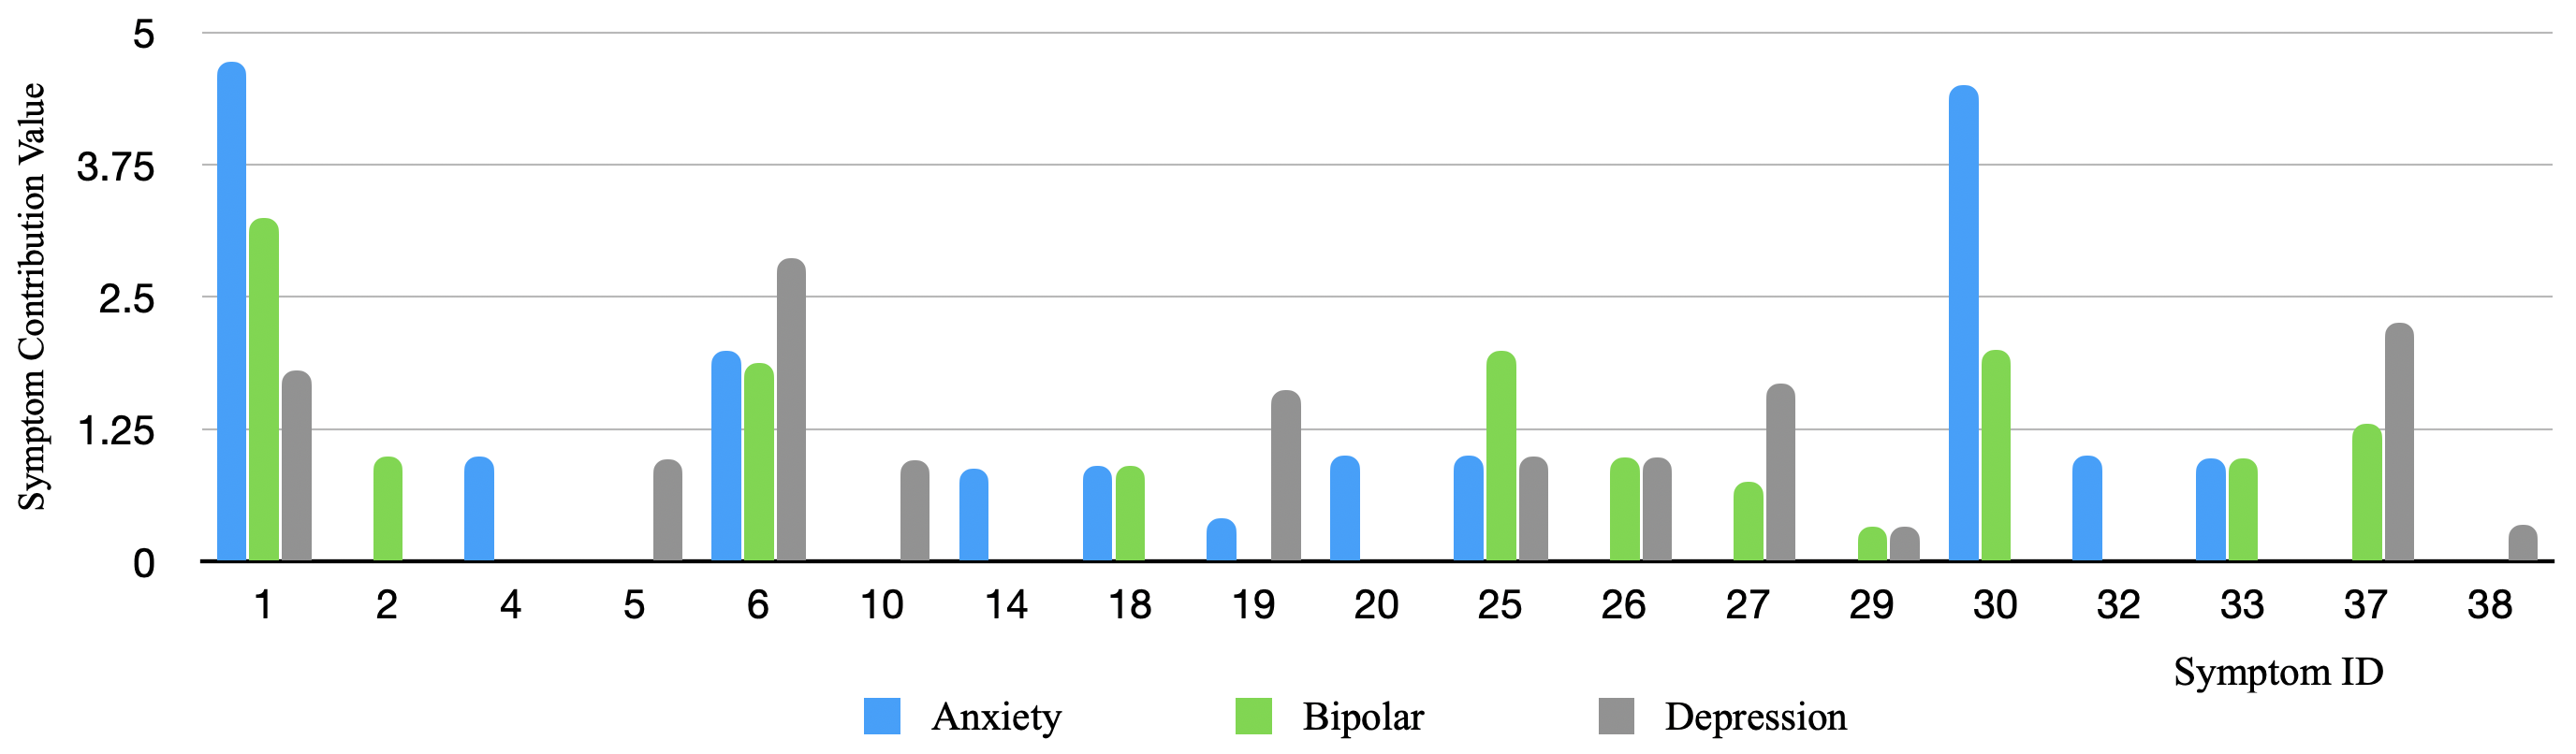
\includegraphics[width=\linewidth]{figures/symptom_stream_score.png}
    \caption{User-level symptom contribution values according to the attention scores obtain from symptom stream model. The user is diagnosed with anxiety, bipolar and depression. We provide the corresponding symptom names with symptom ID in Table \ref{tab:symp_id} (Appendix \ref{apd:symps}), and we omit the symptoms whose contribution values of anxiety, bipolar and depression are all 0.}
    \label{fig:symp_stream_score}
\end{figure*}

\begin{figure*}[th]
    \centering
    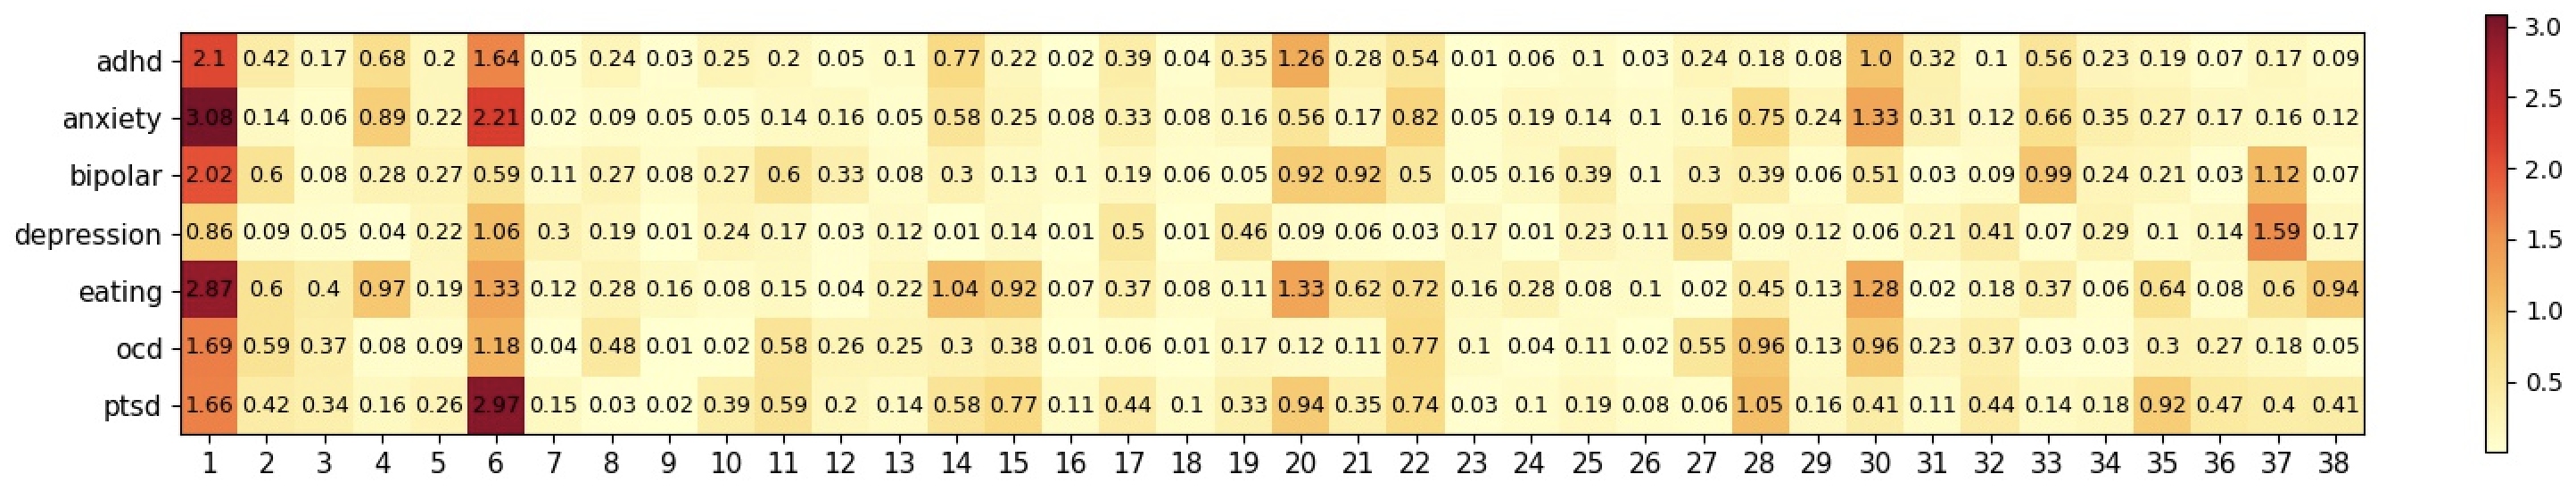
\includegraphics[width=\linewidth]{figures/symp_contributions.png}
    \caption{Global symptom contribution vectors of all users in the test set. We provide the corresponding symptom names with symptom id in Table \ref{tab:symp_id}, Appendix \ref{apd:symps}.}
    \label{fig:symp_contribution}
\end{figure*}

Therefore, we provide a concrete user-level example to illustrate the decision-making process of PsyEx. The selected user suffers from three mental disorders, including \textit{anxiety, bipolar} and \textit{depression}. 
We apply the trained PsyEx model to his/her posting history, and obtain the attention score matrix of symptom stream, which is $D \times N$, since there're $D$ disease-specific attention heads. To figure out which symptoms are more critical for diagnosing a certain disease, we measure the \textit{contribution} of each symptom to the detection of different diseases, with the help of attention score matrix. 

For each diagnosed disease $d$, we calculate the \textbf{symptom contribution vector} $C_d$ as follows. 
First, we select eight symptom probability vectors $S_d = \{s_1, s_2, ..., s_{8}\}$ with the highest attention score among the symptom stream. Next, for each 38-dimensional vector $s_i$, we only preserve the value of three symptoms with highest probability. So we set the probability of rest symptoms to 0 and obtain $\hat{s_i}$. Finally, we can get the user's symptom contribution vector
\begin{equation}
    C_d = \sum_{i=1}^8 \hat{s_i}
    \label{eq:symp_contri}
\end{equation}
which is demonstrated in Figure \ref{fig:symp_stream_score}. 

The symptom contribution vectors of these three mental diseases are quite different from each other, satisfying the first aspect of interpretability (i.e., Difference), which means that our proposed model, to some extent, have learned how to ``diagnose'' a certain disease with its corresponding symptoms just like psychiatrists. 

But do these learned high-contribution symptoms truly make sense for the diagnosis?  We compare our symptom contribution vectors with the standard criteria DSM-5 to validate the second aspect of interpretability (i.e., Reasonableness). 
From Figure~\ref{fig:symp_stream_score}, we can find out that typical symptoms ``6: depressed mood''\footnote{We present the symptoms in ``ID: name'' format.} and ``37: weight and appetite change'' of depression, ``1: anxious mood'' and ``30: panic fear'' of anxiety do contribute more to the detection of them than to other diseases, which is in line with  DSM-5 . Moreover, we can also notice many shared high-contribution symptoms between bipolar disorder and depression, which is reasonable because bipolar disorder contains both depressive episodes and hypomanic episodes\footnote{\url{https://www.nimh.nih.gov/health/topics/bipolar-disorder}}. 
Therefore, we claim that the explicit usage of symptoms, as well as disease-specific attention layers, can exactly improve the interpretability of our neural network model.

\subsection{Global Symptom Contribution Analysis}
To provide a global view of high-contribution symptoms for all the 7 diseases, we plot a heatmap (See Figure \ref{fig:symp_contribution}) of symptom contribution vectors based on all the users in the test set. 
Here, we group the users according to his/her diagnosed diseases, and obtain 7 disease-specific user subsets \footnote{a user with multiple mental diseases is in multiple subsets}. For each disease subset, we calculate all the user-level symptom contribution vectors as \eqnref{eq:symp_contri} based on the attention score, and aggregate them by averaging to get the global contribution vector of each disease. 


% \KZ{When I compare \figref{fig:symp_contribution} with \figref{fig:symp_stream_score}, there seems to be a lot of agreement between the two, then what is the poing of presenting them both? Does it imply that the risky post stream is not that useful? Because adding it doesn't seem to change the weights? I think we need to do some reasoning here.} 

Apart from a lot of agreement reached between our global contribution vector and the authoritative DSM-5 (e.g., ``21: drastical shift in mood and energy'' for bipolar disorder), we can find several interesting inconsistencies. For example, eating disorder patients are ``38: more irritable'' and tend to ``20: do things that easily get painful consequences'', both of which are typical symptoms for bipolar disorder patients in the manic episodes, probably due to the high comorbidity of these two disorders proved by previous researches \cite{LUNDE2009relation, Ruiz2015Comorbidity}. 
Further, almost all the diseases treat ``1: anxious mood'' and ``6: depressed mood'' as the most important symptoms in PsyEx, while in DSM-5, they're not the typical symptoms for diagnosing many mental diseases such as ADHD. We try to explain this as follows. As a diagnostic criteria, DSM-5 tend to focus on the distinctive symptoms of each disease rather than the common ones. However, these common symptoms can be generally meaningful to distinguish patients of most disorders from control users, so they are highly weighted by our PsyEx model. 












% \subsubsection{Risky Post Stream Interpretability}
% The attention score of the risky post stream is a $D \times K$ matrix, indicating which posts are more important for the detection of each disease. 
% Interestingly, we find only minor differences in the distribution of attention score for the 7 diseases, and there‘re three posts whose corresponding attention scores are in the top-5 of all the diagnosed diseases, so we simply show these posts and their symptoms in \tabref{tab:example}.   

% \footnote{We provide the symptoms of 7 mental disorders (Table \ref{tab:symp_of_dsm5}) extracted from DSM-5 in Appendix \ref{apd:symp_contribution} for reference.}. 


% For each user with disease $d$, we only select 16 symptom vectors $S = \{s_1, s_2, ..., s_{16}\}$ with highest attention score, and add them to the symptom contribution vector. 
% Finally, we normalized the symptom contribution vectors by dividing the number of users with each disease, and demonstrate them in a heat map (Figure \ref{fig:symp_contribution}) for all the diseases\footnote{We also provide another heat map (Figure \ref{fig:symp_contribution_wo_attn}) calculated without the assistance of attention score in Appendix \ref{apd:symp_contribution}.}.
% Here, we use serial numbers to represent symptoms, and provide the corresponding symptom names in Table \ref{tab:symp_id} (Appendix \ref{apd:symp_contribution}). 

% In Figure \ref{fig:symp_contribution}, we can work out which symptoms are more critical for diagnosing a certain disease. The typical symptom "6: depressed mood"\footnote{We present the symptoms in "ID: name" format.} of depression, "1: anxious mood" of anxiety, and "11: Inattention" of ADHD exactly contributes more to the detection of them than to other diseases, which is in line with DSM-5 criteria\footnote{We provide the symptoms of 7 mental disorders (Table \ref{tab:symp_of_dsm5}) extracted from DSM-5 in Appendix \ref{apd:symp_contribution} for reference.}. 
% 
% \KZ{Rephrase this: ``do things easily get painful consequences''}, 
% \KZ{Is this a userful discovery?}
% \MYW{Consider making a figure containing posts along with disease prediction (multiple tags) and their corresponding symptoms}

% PsyEx suggests that "anxious mood", "depressed mood" is the most important symptoms for PSTD diagnosis, while "intrusion symptoms" and "avoidance of stimuli", two more PTSD-specific symptoms described in DSM-5, gets relatively lower attention in our model. That's probably because these two "mood" symptoms exists more common in the users' posts.  


